\nonstopmode

\title{Row-level MAC in H2}
\author{Christopher Martin\\{\tt chris.martin@gatech.edu}}

\documentclass[twocolumn]{article}

\usepackage{hyperref}\hypersetup{hidelinks}
\usepackage{graphicx}
\usepackage{verbatim}
\usepackage{fullpage}

\begin{document}

\twocolumn[
  \begin{@twocolumnfalse}
    \maketitle
    \begin{abstract}
      This project explores how a relational database manager can be modified to enforce a mandatory access control policy (MAC) using a multi-level security (MLS) model. The prototype I built from the H2 DBMS enforces read permissions on a per-tuple granularity and includes security-related additions to the SQL grammar.
      ~\\
    \end{abstract}
  \end{@twocolumnfalse}
]

\section{Motivation}

The aim is to help provide strong guarantees for information protection in information systems. In particular I consider the requirements of the U.S. Department of Defense, but the results are conceivably generalizable to other areas such as the healthcare industry.

\section{Security model}

Here we consider a slightly simplified variant of the U.S. Department of Defense multilevel security (MLS) model.

\begin{description}

  \item[Sensitivity level] A fully ordered set of labels. Herein we call these labels $0$, $1$, $2$, and $3$, where the infimum level $0$ denotes the least sensitive data, and the supremum level $3$ is applied to the most highly-guarded secrets.

  \item[Compartment] A set of labels indicating topics to which data pertains. This set is partially ordered because topics may be nested hierarchically. For example, if the compartment {\it Food} contains the compartments {\it Apples} and {\it Oranges}, then ${\it Food} > {\it Bananas}$, but {\it Apples} and {\it Oranges} are incomparable.

  \item[Marking] A marking consists of one sensitivity level and any number of compartments. We denote this by separating the components with slashes, such as {\it 2/Apples/Bananas}. Markings form a lattice where the infinum is {\it 0} and the supremum is a marking with the highest sensitivity and every compartment.

  \item[Credential] A credential consists of a sensitivity level and a compartment. Each subject has a set of credentials.

\end{description}

A subject has read access to data marked by {\it $\ell$/$C_1$/$C_2$/\ldots/$C_n$} only if for all $i \in [1, n]$ the subject has a credential ($\ell'$, $C'$) such that $\ell' \ge \ell$ and $C' \ge C_i$.

\begin{figure}
  \begin{center}
    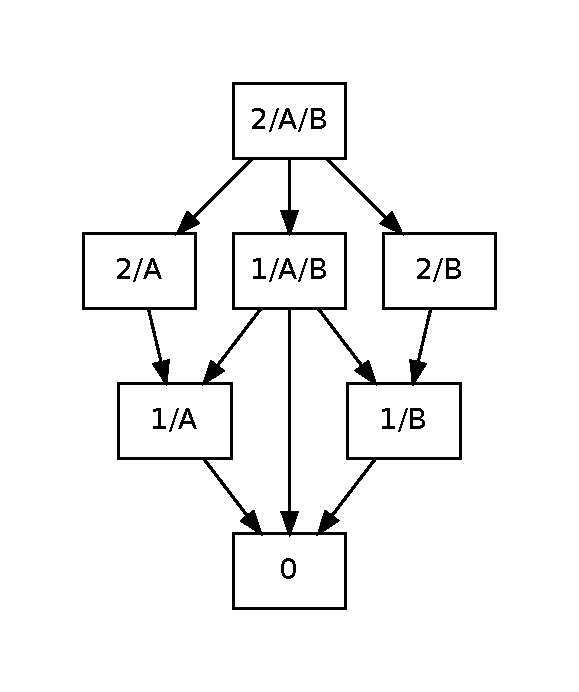
\includegraphics[width=0.75\linewidth]{lattice.pdf}
  \end{center}
  \caption{........}

  \label{fig:lattice}
\end{figure}

\section{Implementation}

The deliverable will be a modified version of H2\cite{h2}, an open source pure-Java DBMS.

\begin{figure*}
  \begin{center}
    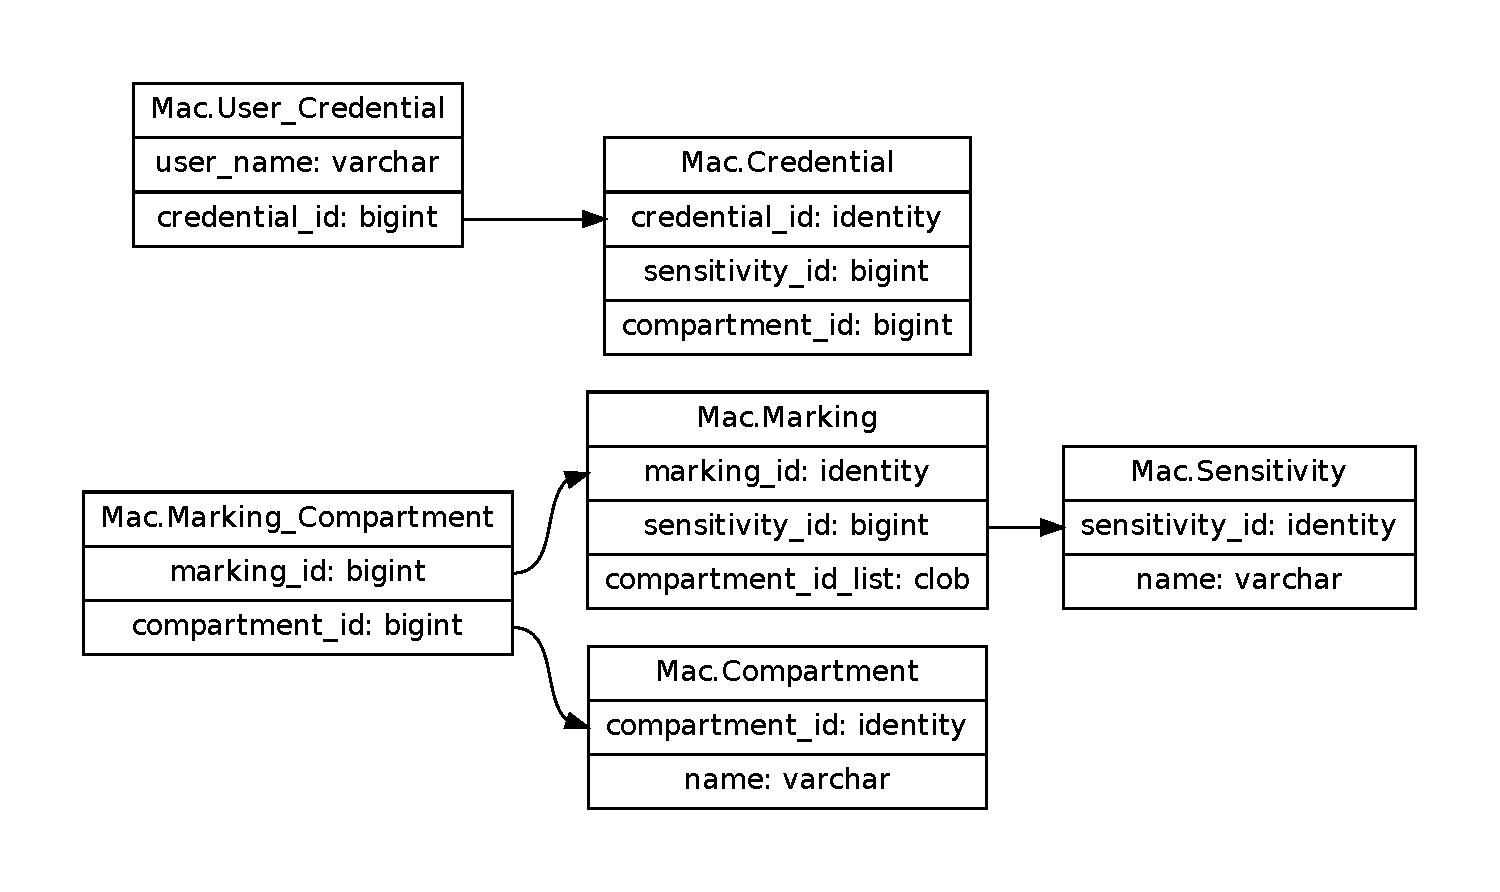
\includegraphics[width=\linewidth]{mac-schema.pdf}
  \end{center}
\end{figure*}

H2's internal schema consists of {\tt MetaTable}s, one of which is for {\tt User}s. This schema will need to be extended to store user credentials. A user with the {\it modify-credentials} {\tt Role} will be able to invoke a built-in procedure to modify users' credentials.

One candidate idea to achieve information hiding is to shadow every {\tt Table} with a {\tt TableView} that selects only rows that the user is allowed to access. When the connection is first established, we can use the user's credentials and the compartment hierarchy to fill a metatable of credentials that the user does {\it not} have. With that set precomputed, it should be possible to generate each table's view by selecting all rows that do not require those credentials.

Oracle has a similar extension to Oracle Database called Oracle Label Security (OLS)\cite{ols} which may serve as inspiration.

\section{Evaluation plan}

\begin{figure}
  \begin{center}
    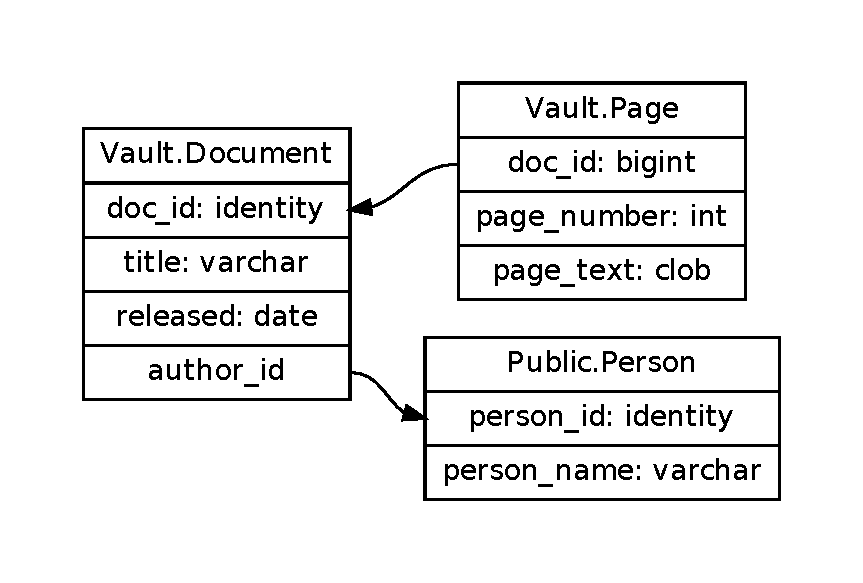
\includegraphics[width=\linewidth]{test-schema.pdf}
  \end{center}
  \caption{........}

  \label{fig:lattice}
\end{figure}

The test setup models a system for storing multi-page documents.

The {\tt Document} and {\tt Page} tables are both separately protected with markings, so a user who can see a document may not be able to see all of its pages.

\paragraph{Correctness}

The foremost question will be whether the security properties hold, which is a simple matter of applying various document and page markings and verifying that {\tt select} queries executed by different database users return appropriate subsets of the data.

\paragraph{Performance}

Performance evaluation will test {\tt insert} and {\tt select} queries to answer two questions:

\begin{itemize}
\item What is the base cost incurred by enabling security in the most trivial case where all tuples are marked with the minimum sensitivity and no compartments?
\item How does performance scale as a function of the number of tuples and the number of security compartments, in comparison with the same system without the security feature?
\end{itemize}

\end{description}

\bibliographystyle{plainnat}
\begin{thebibliography}{99}
\bibitem{h2}{H2 database. \url{http://h2database.com/}}
\bibitem{ols}{Oracle Label Security. \url{http://www.oracle.com/us/products/database/options/label-security/overview/index.html}}
\bibitem{tcsec}{Department of Defense. 1985. {\it Trusted Computer System Evaluation Criteria} (Orange Book). ``Division B: Mandatory protection''}
\end{thebibliography}

\end{document}
